\documentclass{beamer}
\usepackage[utf8]{inputenc}
\usepackage[squaren]{SIunits}
\usepackage{varwidth,setspace}
\usepackage{tikz}
\usetikzlibrary{intersections,positioning,backgrounds,fit,matrix,shapes,calc,decorations.pathmorphing,decorations.text}
\usetheme{default}

\newcommand*{\mimg}[2]{\begingroup
\setbox0=\hbox{\includegraphics[height=#2]{#1}}\parbox{\wd0}{\box0}\endgroup}
\newcommand*{\symok}[0]{
\includegraphics[height=1em]{symbol_ok.pdf}}
\newcommand*{\symbad}[0]{
\includegraphics[height=1em]{symbol_bad.pdf}}
\newcommand*{\symidk}[0]{{\bf\color{blue}\Large?}}

\setbeamertemplate{navigation symbols}{}%remove navigation symbols
\setbeamertemplate{footline}{\hspace*{.5cm}\scriptsize{\hfill\raisebox{1mm}{\insertframenumber}\hspace*{.5cm}}}

\setlength{\tabcolsep}{0.5mm}

\title{Measuring B-modes}
\author{Sigurd Kirkevold Næss}
\institute{Subdepartment of astrophysics, Oxford University}
\date{September 9th, 2014}

\begin{document}

\begin{frame}
	\titlepage
\end{frame}

\begin{frame}{From pristine CMB to dirty data}
	\begin{center}
		\large%
		\only<1>{At the surface of last scattering}%
		\only<2>{Lensing by large-scale structure}%
		\only<3>{Dusty galaxies, radio sources, SZ clusters}%
		\only<4>{Faraday rotation}%
		\only<5>{Galctic dust, synchrotron, etc}%
		\only<6>{Atmospheric emission}%
		\only<7>{Absolute polarization offset ($1^\circ$ example)}%
		\only<8>{Telescope optics (w. sidelobe)}%
		\only<9>{Detector noise}%
		\only<10>{Glitches}%
		\uncover<1-0>{()}% Dummy to keep line height constant
	\end{center}
	\begin{tikzpicture}[thick,red,decoration={snake, amplitude=1mm,segment length = 5mm}]
		\node at (0.0,0) (A) {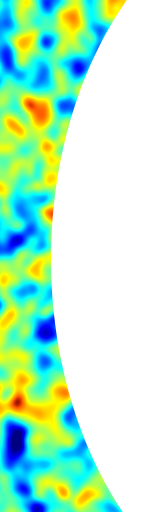
\includegraphics[height=1cm]{sls.png}};
		\node at (2.5,0) (B) {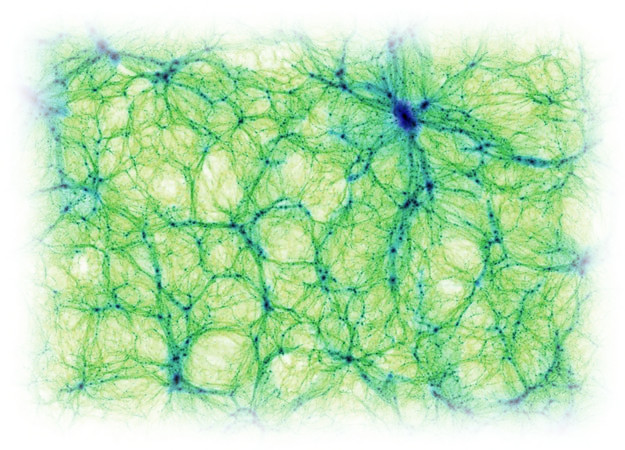
\includegraphics[height=1.5cm]{lss.jpeg}};
		\node at (5.0,0) (C) {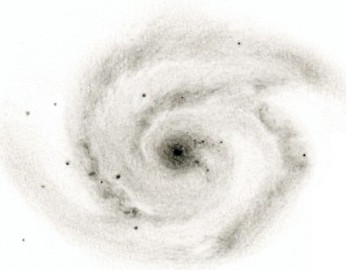
\includegraphics[height=1cm]{galaxy.jpeg}};
		\node at (7.5,0) (D) {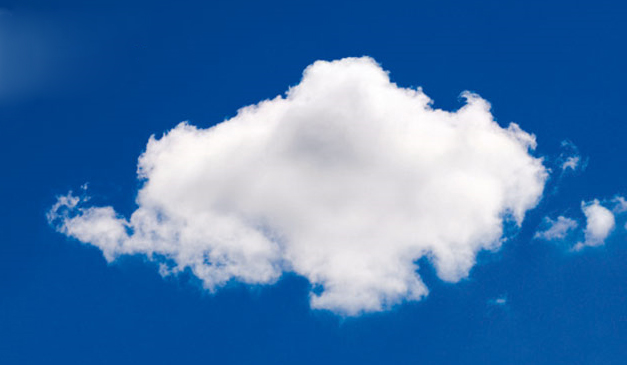
\includegraphics[height=1cm]{cloud.jpg}};
		\node at (10.0,0) (E) {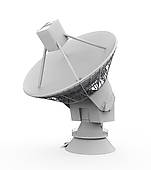
\includegraphics[height=1cm]{telescope.jpg}};
		\only<1>{\draw [decorate] (0,0) -- (0.5,0);}%
		\only<2-3>{\draw [decorate] (0,0) -- (2.5,0);}%
		\only<4-5>{\draw [decorate] (0,0) -- (5.0,0);}%
		\only<6>{\draw [decorate] (0,0) -- (7.5,0);}%
		\only<7-10>{\draw [decorate] (0,0) -- (10.0,0);}%
	\end{tikzpicture}
	\hspace*{-5mm}\begin{tabular}{ccc}
		T&E&B\\
	\only<1>{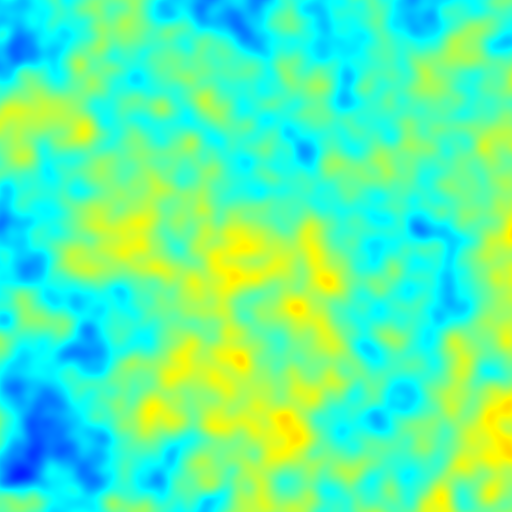
\includegraphics[width=0.35\textwidth]{out_dirty/01_cmb_teb_0.png}}%
	\only<2>{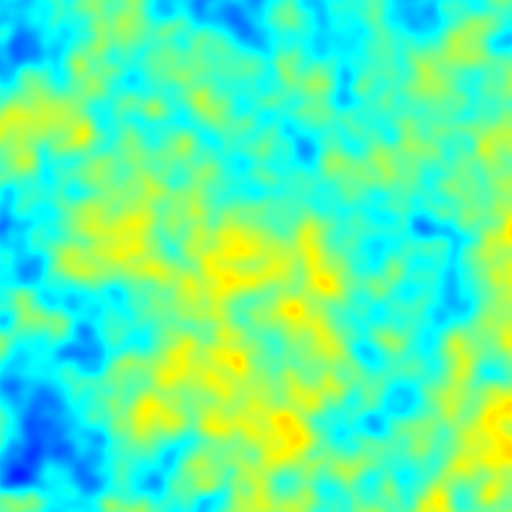
\includegraphics[width=0.35\textwidth]{out_dirty/02_lens_teb_0.png}}%
	\only<3>{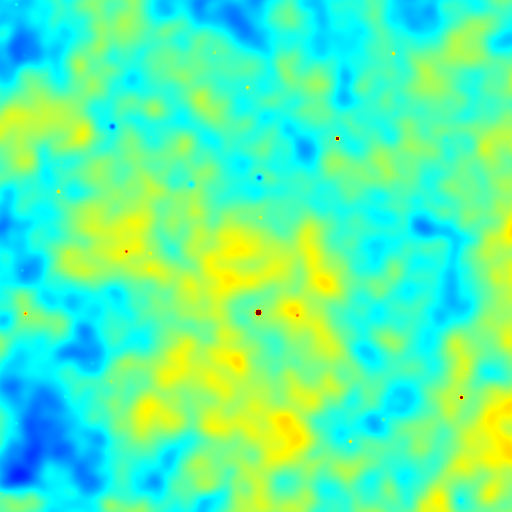
\includegraphics[width=0.35\textwidth]{out_dirty/04_sz_teb_0.png}}%
	\only<4>{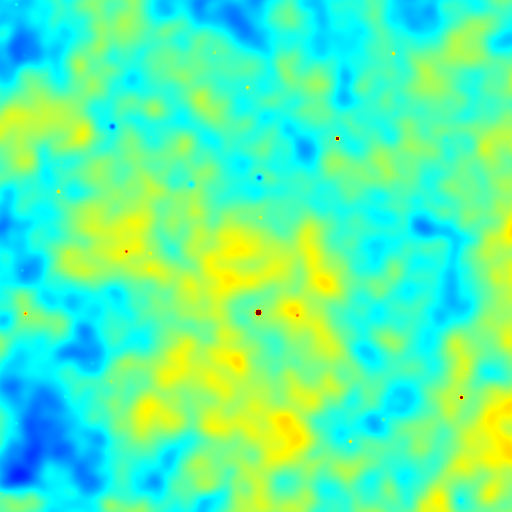
\includegraphics[width=0.35\textwidth]{out_dirty/05_faraday_teb_0.png}}%
	\only<5>{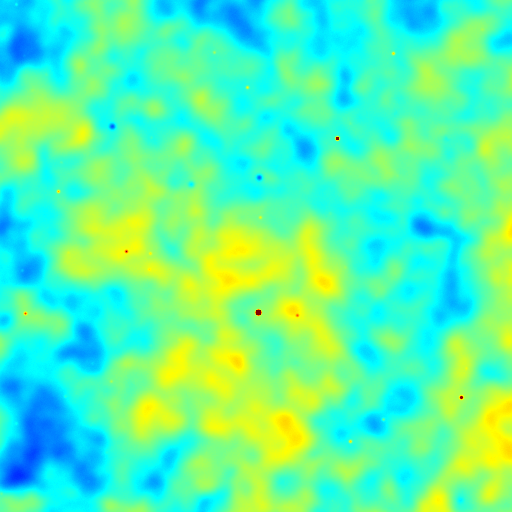
\includegraphics[width=0.35\textwidth]{out_dirty/06_dust_teb_0.png}}%
	\only<6>{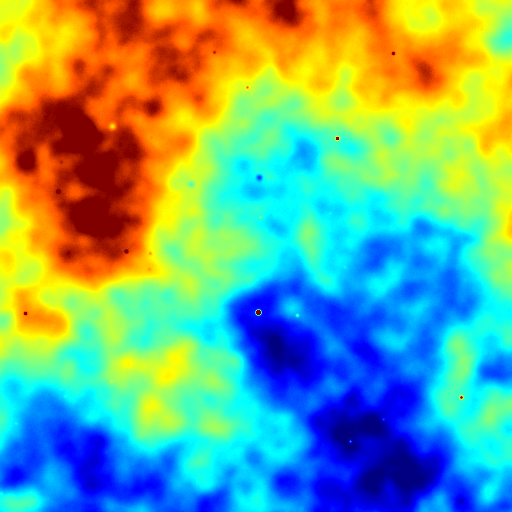
\includegraphics[width=0.35\textwidth]{out_dirty/07_atm_teb_0.png}}%
	\only<7>{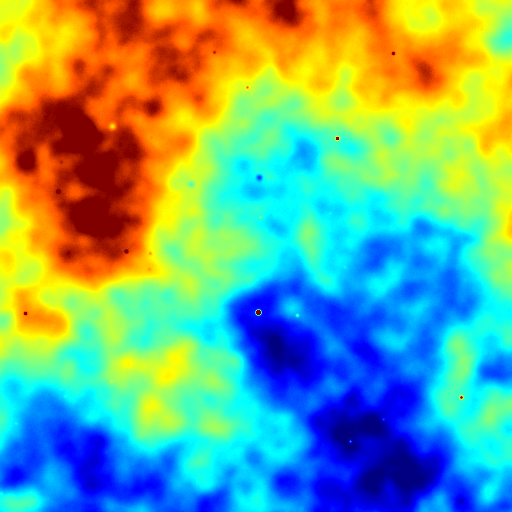
\includegraphics[width=0.35\textwidth]{out_dirty/08_polerr_teb_0.png}}%
	\only<8>{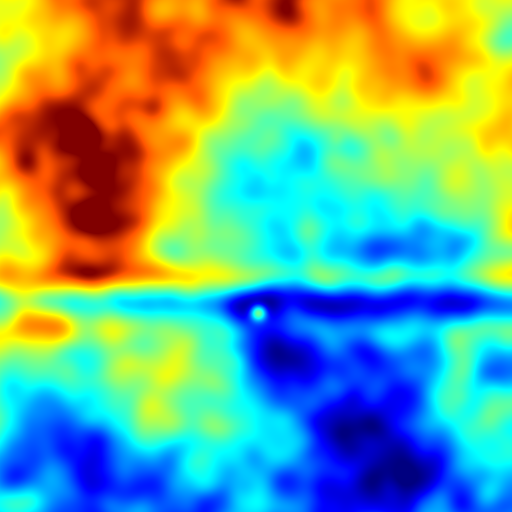
\includegraphics[width=0.35\textwidth]{out_dirty/10_beam_teb_0.png}}%
	\only<9>{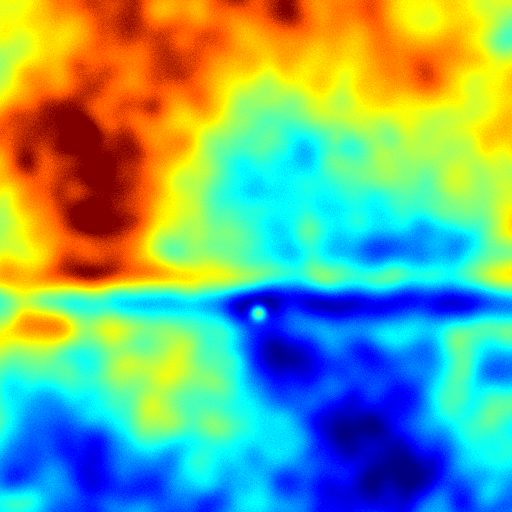
\includegraphics[width=0.35\textwidth]{out_dirty/11_noise_teb_0.png}}%
	\only<10>{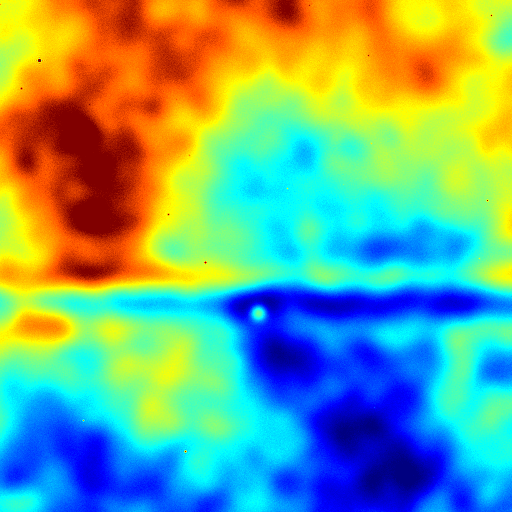
\includegraphics[width=0.35\textwidth]{out_dirty/12_glitch_teb_0.png}}%
	&
	\only<1>{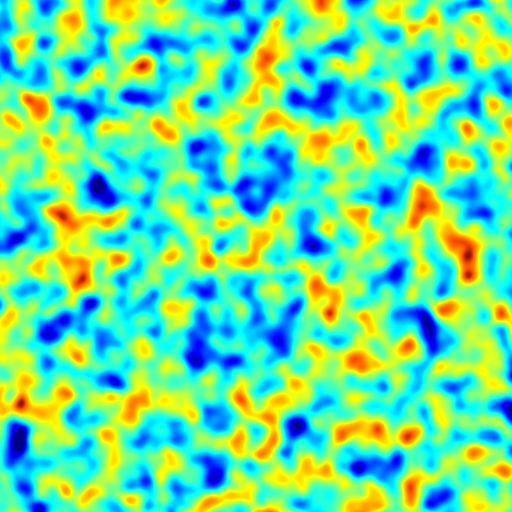
\includegraphics[width=0.35\textwidth]{out_dirty/01_cmb_teb_1.png}}%
	\only<2>{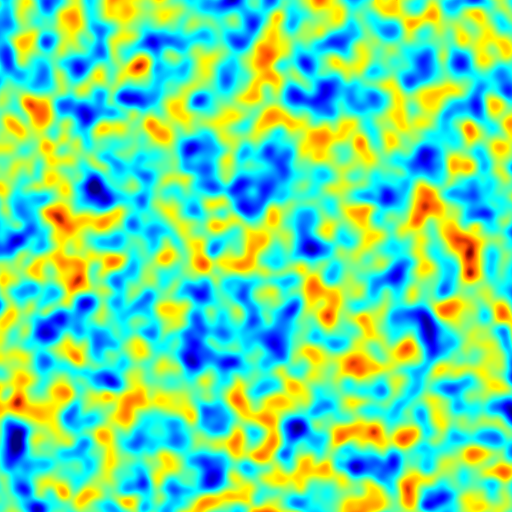
\includegraphics[width=0.35\textwidth]{out_dirty/02_lens_teb_1.png}}%
	\only<3>{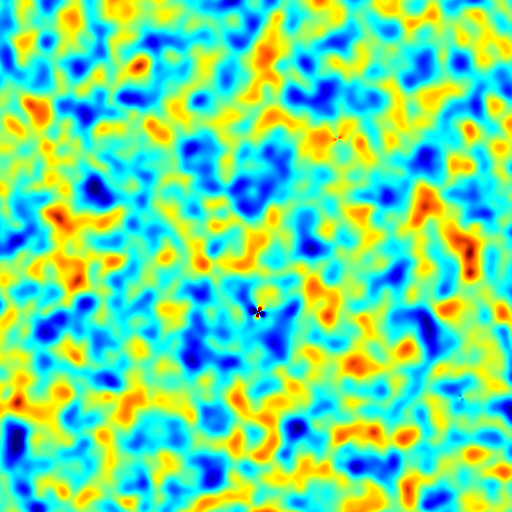
\includegraphics[width=0.35\textwidth]{out_dirty/04_sz_teb_1.png}}%
	\only<4>{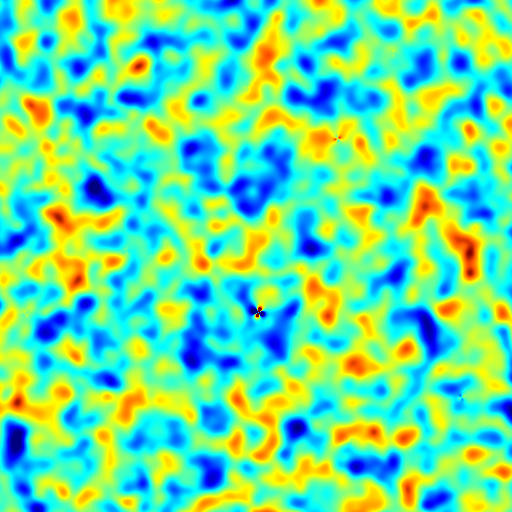
\includegraphics[width=0.35\textwidth]{out_dirty/05_faraday_teb_1.png}}%
	\only<5>{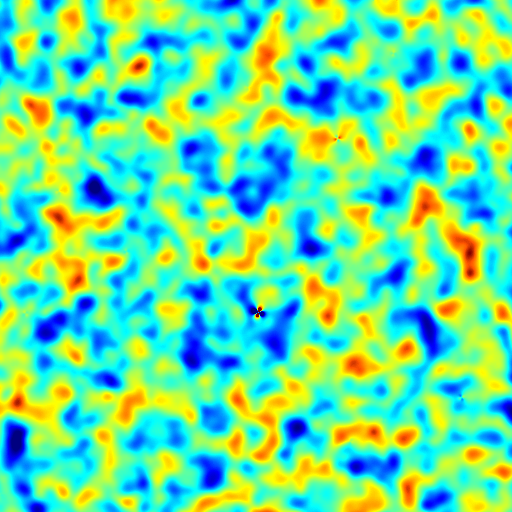
\includegraphics[width=0.35\textwidth]{out_dirty/06_dust_teb_1.png}}%
	\only<6>{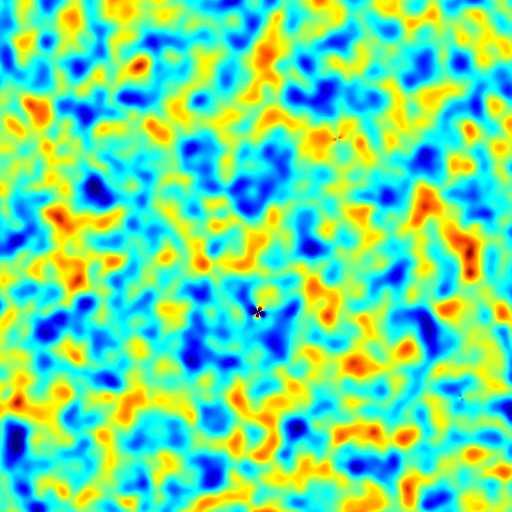
\includegraphics[width=0.35\textwidth]{out_dirty/07_atm_teb_1.png}}%
	\only<7>{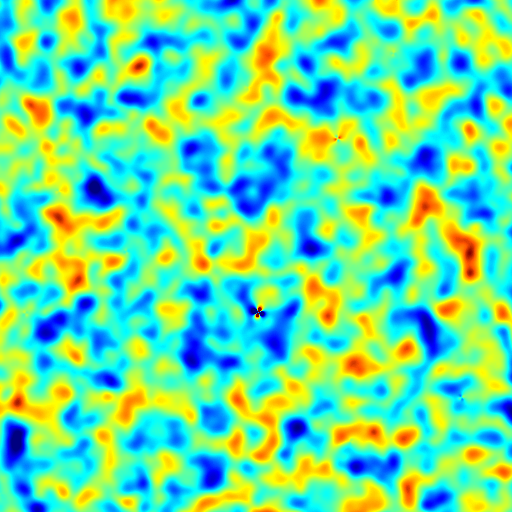
\includegraphics[width=0.35\textwidth]{out_dirty/08_polerr_teb_1.png}}%
	\only<8>{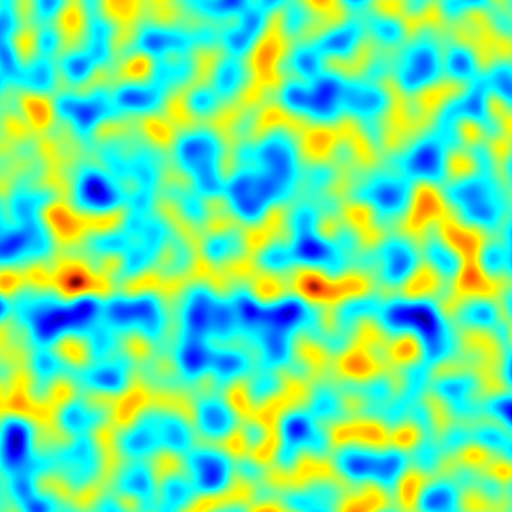
\includegraphics[width=0.35\textwidth]{out_dirty/10_beam_teb_1.png}}%
	\only<9>{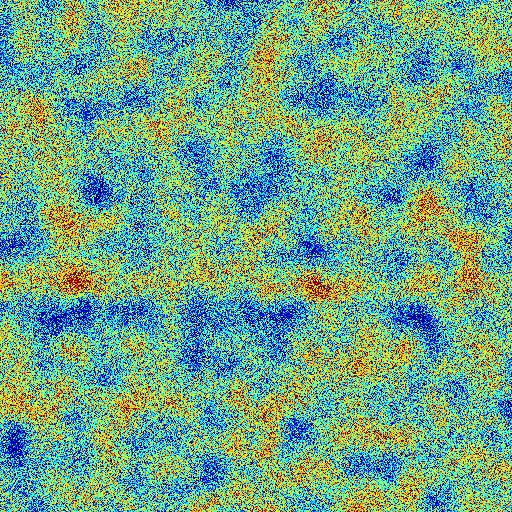
\includegraphics[width=0.35\textwidth]{out_dirty/11_noise_teb_1.png}}%
	\only<10>{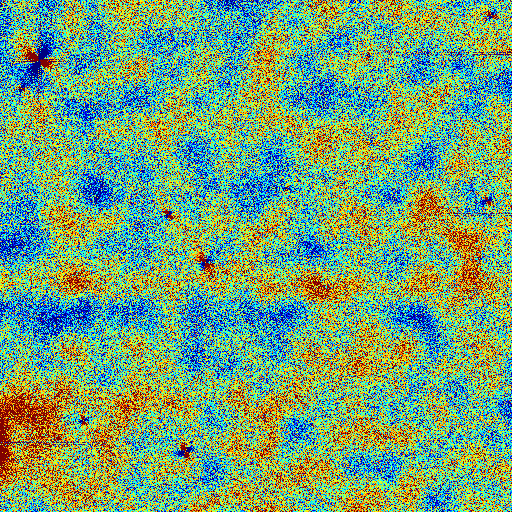
\includegraphics[width=0.35\textwidth]{out_dirty/12_glitch_teb_1.png}}%
	&
	\only<1>{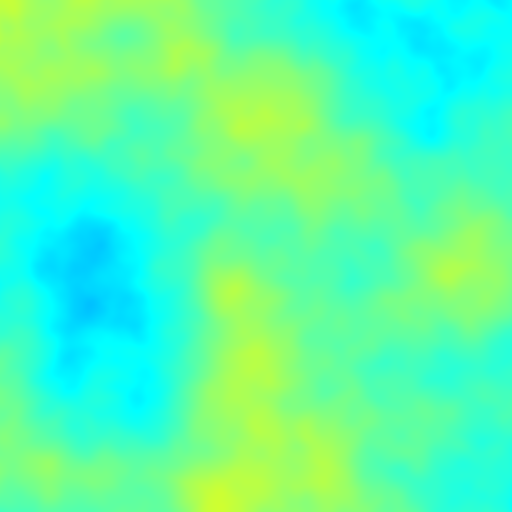
\includegraphics[width=0.35\textwidth]{out_dirty/01_cmb_teb_2.png}}%
	\only<2>{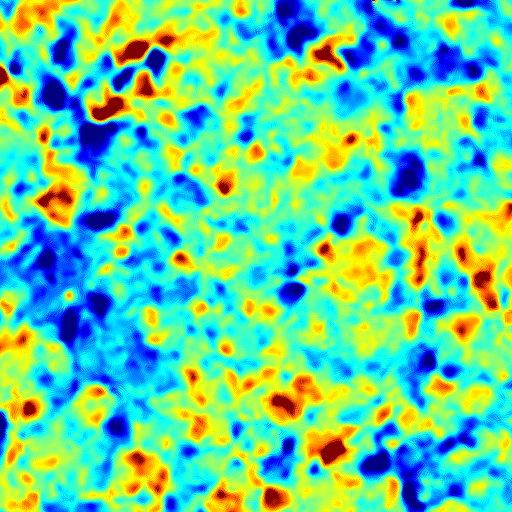
\includegraphics[width=0.35\textwidth]{out_dirty/02_lens_teb_2.png}}%
	\only<3>{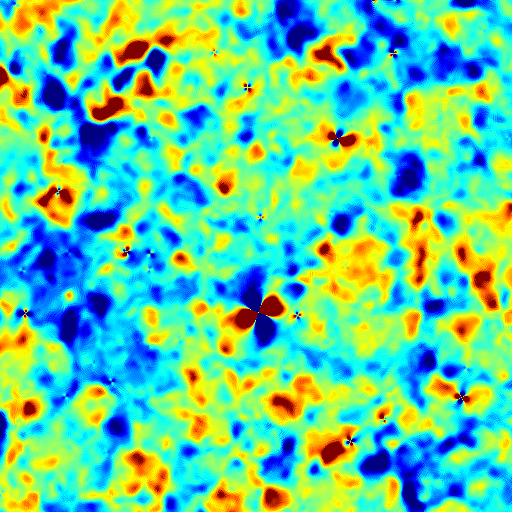
\includegraphics[width=0.35\textwidth]{out_dirty/04_sz_teb_2.png}}%
	\only<4>{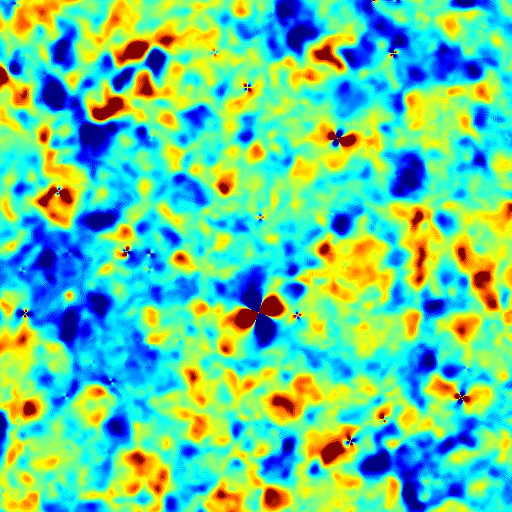
\includegraphics[width=0.35\textwidth]{out_dirty/05_faraday_teb_2.png}}%
	\only<5>{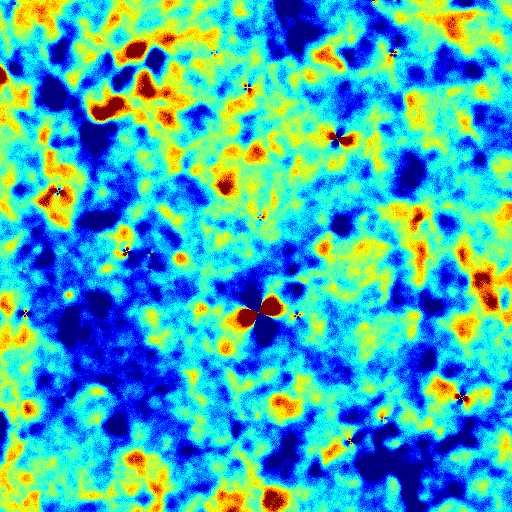
\includegraphics[width=0.35\textwidth]{out_dirty/06_dust_teb_2.png}}%
	\only<6>{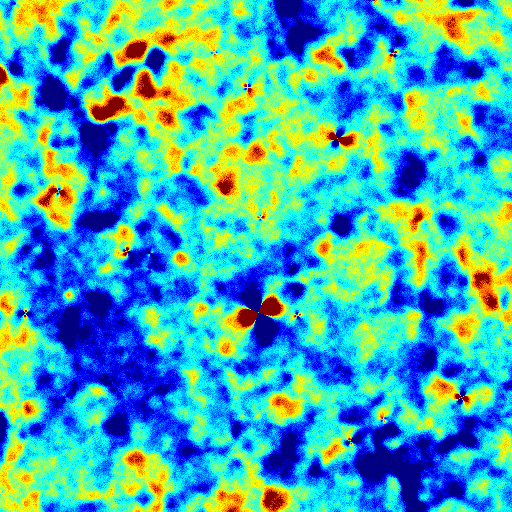
\includegraphics[width=0.35\textwidth]{out_dirty/07_atm_teb_2.png}}%
	\only<7>{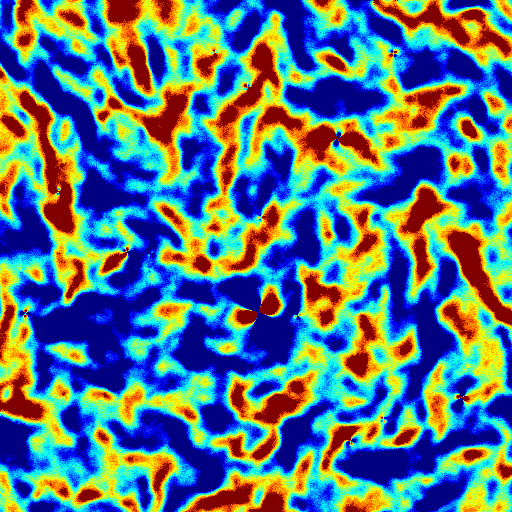
\includegraphics[width=0.35\textwidth]{out_dirty/08_polerr_teb_2.png}}%
	\only<8>{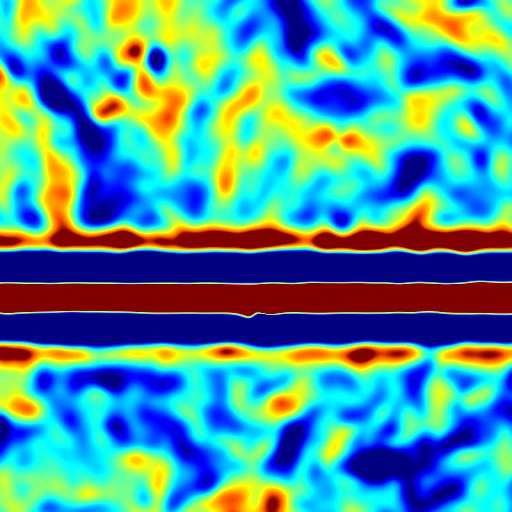
\includegraphics[width=0.35\textwidth]{out_dirty/10_beam_teb_2.png}}%
	\only<9>{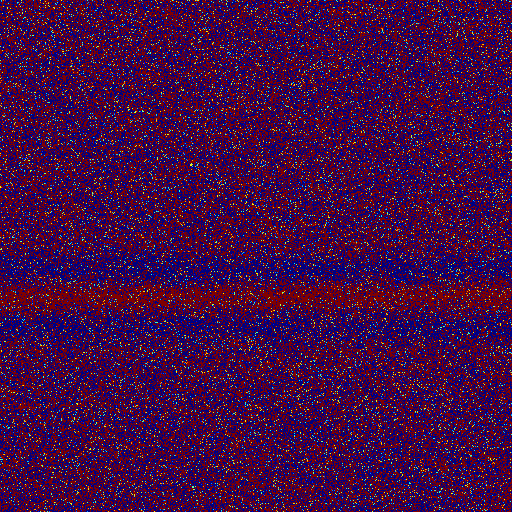
\includegraphics[width=0.35\textwidth]{out_dirty/11_noise_teb_2.png}}%
	\only<10>{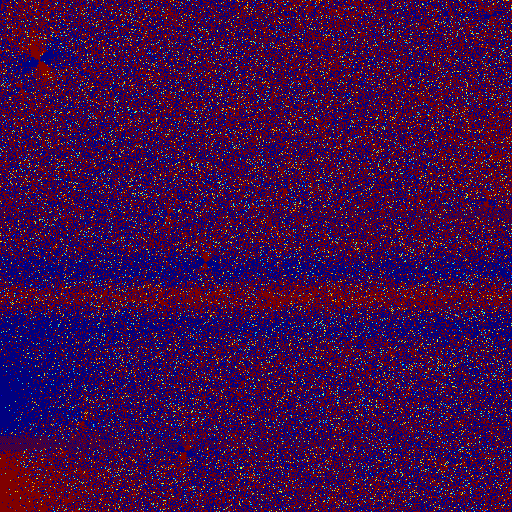
\includegraphics[width=0.35\textwidth]{out_dirty/12_glitch_teb_2.png}}%
	\\
	{\footnotesize $-500\mu$K\enskip
\includegraphics[width=12mm,height=2mm]{colorbar.png}\enskip$500\mu$K} &
	{\footnotesize $-20\mu$K\enskip
\includegraphics[width=12mm,height=2mm]{colorbar.png}\enskip$20\mu$K} &
	{\footnotesize $-1\mu$K\enskip
\includegraphics[width=12mm,height=2mm]{colorbar.png}\enskip$1\mu$K}
\end{tabular}\hspace*{-5mm}
\end{frame}

\begin{frame}{What the telescope actually observes}
	\begin{tikzpicture}[bad/.style={line width=3pt,red}]
		\node at (0,0) {\begin{tabular}{ccc}
				T & E & B \\
				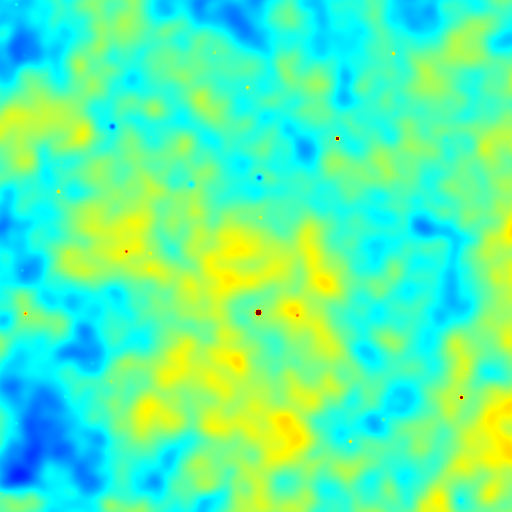
\includegraphics[width=0.30\textwidth]{out_dirty/04_sz_teb_0.png} &
				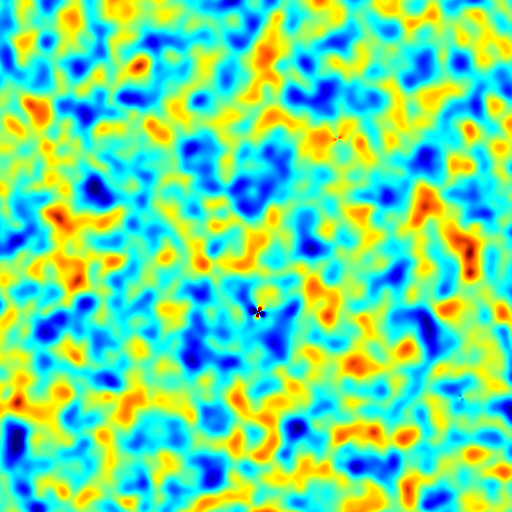
\includegraphics[width=0.30\textwidth]{out_dirty/04_sz_teb_1.png} &
				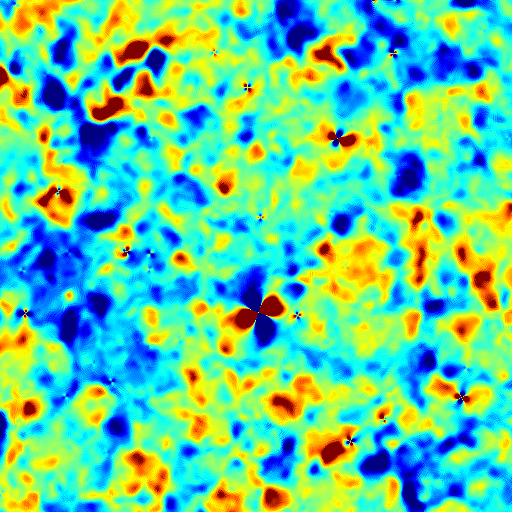
\includegraphics[width=0.30\textwidth]{out_dirty/04_sz_teb_2.png}
		\end{tabular}};
		\draw[bad] (-5, 1.5) -- (5,-1.8);
		\draw[bad] (-5,-1.8) -- (5, 1.5);
		\node at (0,-4) {\begin{tabular}{ccc}
				\only<1-2>{T+pol}\only<3->{T} & \uncover<3->{Q} & \uncover<3->{U} \\
				\only<1-2>{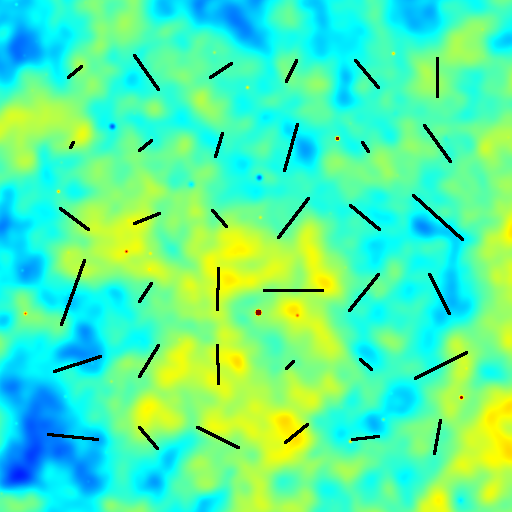
\includegraphics[width=0.30\textwidth]{out_dirty/t_polvec.png}}%
				\only<3->{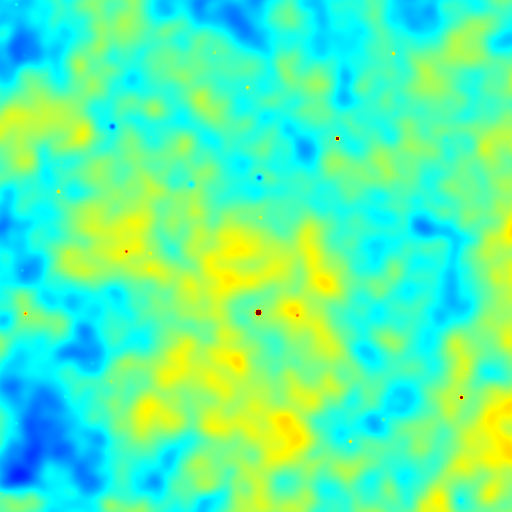
\includegraphics[width=0.30\textwidth]{out_dirty/04_sz_tqu_0.png}} &
				\uncover<3->{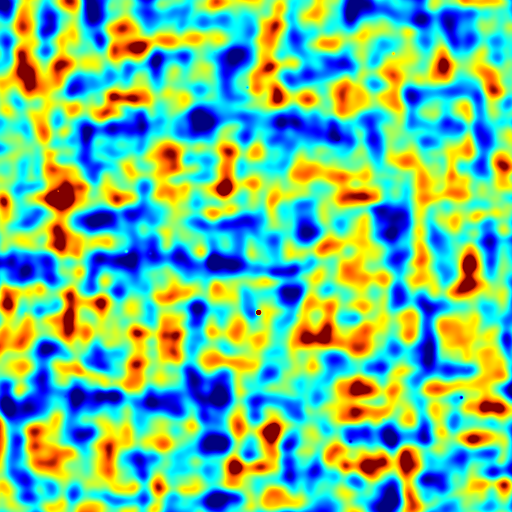
\includegraphics[width=0.30\textwidth]{out_dirty/04_sz_tqu_1.png}} &
				\uncover<3->{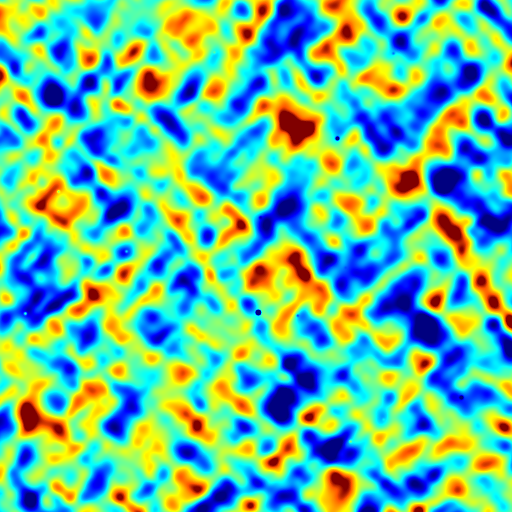
\includegraphics[width=0.30\textwidth]{out_dirty/04_sz_tqu_2.png}}
		\end{tabular}};
		\uncover<2>{\node at (1.5,-4) {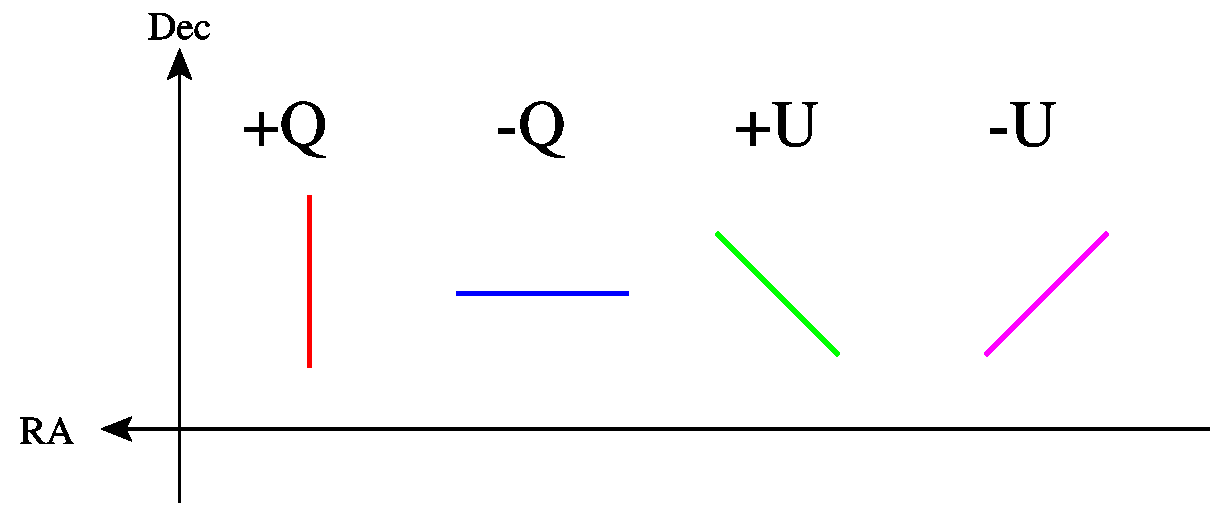
\includegraphics[height=3cm]{qudef.pdf}};}
	\end{tikzpicture}
\end{frame}

\begin{frame}{E, B and Q, U}
	\begin{center}
		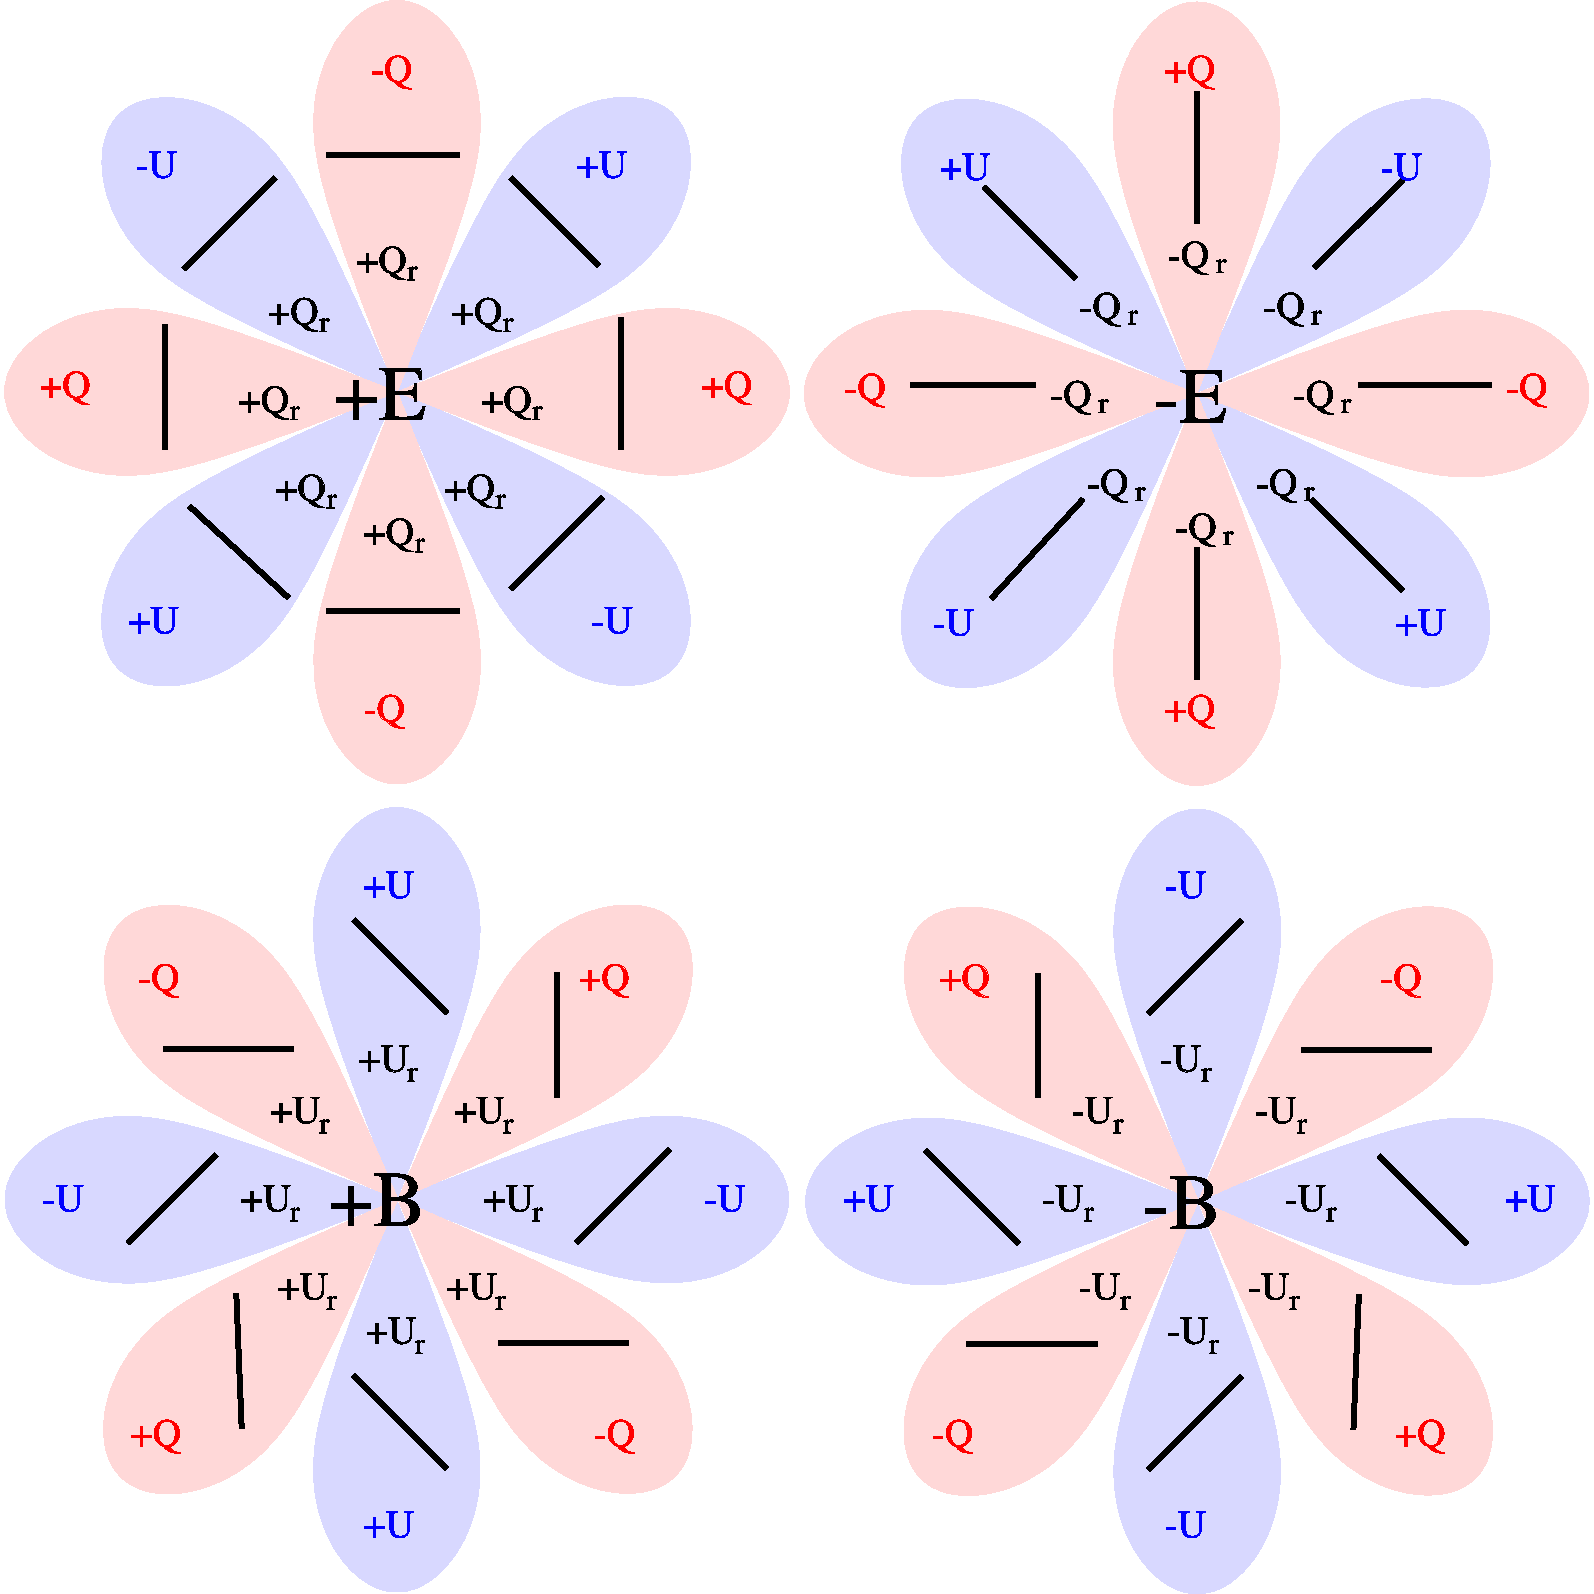
\includegraphics[height=8cm]{EB_iau.pdf}
	\end{center}
\end{frame}

\begin{frame}{Actually only observe linear combinations}
	\begin{center}
	\begin{tabular}{c}
		\only<1>{Detector 1: T+Q}%
		\only<2>{Detector 2: T+U}%
		\only<3>{Detector 3: T-Q}%
		\only<4>{Detector 4: T-U}%
		\\
		\only<1>{\includegraphics[height=7cm]{out_dirty/tqu_lincombs_0.png}}%
		\only<2>{\includegraphics[height=7cm]{out_dirty/tqu_lincombs_1.png}}%
		\only<3>{\includegraphics[height=7cm]{out_dirty/tqu_lincombs_2.png}}%
		\only<4>{\includegraphics[height=7cm]{out_dirty/tqu_lincombs_3.png}}%
	\end{tabular}
\end{center}
\end{frame}

\begin{frame}{Not like a digital camera}
	\begin{tikzpicture}[bad/.style={line width=8pt,red},scan/.style={thick,red}]
		\node at (0,0) (A) {\includegraphics[height=3cm]{out_dirty/06_dust_teb_0.png}};
		\uncover<2->{%
		\node at (1.5,-1) (B) {\includegraphics[height=3cm]{camera.png}};}
		\uncover<3->{%
		\draw[bad] (-1.1,-2.1) -- ( 2.6, 1.6);
		\draw[bad] (-1.1, 1.6) -- ( 2.6,-2.1);}
		\uncover<4->{%
		\node at (6,0) (C) {\includegraphics[height=3cm]{out_dirty/06_dust_teb_0.png}};}
		\uncover<5->{%
		\draw[scan] (5, 1.0) -- (7, 0.9);}
		\uncover<6->{%
		\draw[scan] (7, 0.9) -- (5, 0.8);}
		\uncover<7->{%
		\draw[scan] (5, 0.8) -- (7, 0.7);}
		\uncover<8->{%
		\draw[scan] (7, 0.7) -- (5, 0.6);}
		\uncover<9->{%
		\draw[scan] (5, 0.6) -- (7, 0.5);}
		\uncover<10->{%
		\draw[scan] (7, 0.5) -- (5, 0.4);}
		\uncover<11->{%
		\draw[scan] (5, 0.4) -- (7, 0.3);
		\draw[scan] (7, 0.3) -- (5, 0.2);
		\draw[scan] (5, 0.2) -- (7, 0.1);
		\draw[scan] (7, 0.1) -- (5, 0.0);
		\draw[scan] (5, 0.0) -- (7,-0.1);
		\draw[scan] (7,-0.1) -- (5,-0.2);
		\draw[scan] (5,-0.2) -- (7,-0.3);
		\draw[scan] (7,-0.3) -- (5,-0.4);
		\draw[scan] (5,-0.4) -- (7,-0.5);
		\draw[scan] (7,-0.5) -- (5,-0.6);
		\draw[scan] (5,-0.6) -- (7,-0.7);
		\draw[scan] (7,-0.7) -- (5,-0.8);
		\draw[scan] (5,-0.8) -- (7,-0.9);
		\draw[scan] (7,-0.9) -- (5,-1.0);
	\draw[scan] (5,-1.0) -- (7,-1.1);}
		\uncover<4->{
		\node at (7.5,-1) (D) {\includegraphics[height=3cm]{telescope2.png}};}
		\uncover<5->{%
		\draw[thick,red,->,rounded corners=1mm] (7.5,-2.4) -- (7.5,-2.6) -- (-0.5,-2.6) -- (-0.5,-2.9);
		\node at (-0.5,-3.00) {\includegraphics[height=0.7mm,width=1.5cm]{out_dirty/scanrow100.png}};}
		\uncover<6->{%
		\node at ( 1.0,-3.00) {\includegraphics[height=0.7mm,width=1.5cm]{out_dirty/scanrow116.png}};}
		\uncover<7->{%
		\node at ( 2.5,-3.00) {\includegraphics[height=0.7mm,width=1.5cm]{out_dirty/scanrow132.png}};}
		\uncover<8->{%
		\node at ( 4.0,-3.00) {\includegraphics[height=0.7mm,width=1.5cm]{out_dirty/scanrow148.png}};}
		\uncover<9->{%
		\node at ( 5.5,-3.00) {\includegraphics[height=0.7mm,width=1.5cm]{out_dirty/scanrow164.png}};}
		\uncover<10->{%
		\node at ( 7.0,-3.00) {\includegraphics[height=0.7mm,width=1.5cm]{out_dirty/scanrow180.png}};}
		\uncover<11->{
		\node at (-0.5,-3.15) {\includegraphics[height=0.7mm,width=1.5cm]{out_dirty/scanrow196.png}};
		\node at ( 1.0,-3.15) {\includegraphics[height=0.7mm,width=1.5cm]{out_dirty/scanrow212.png}};
		\node at ( 2.5,-3.15) {\includegraphics[height=0.7mm,width=1.5cm]{out_dirty/scanrow228.png}};
		\node at ( 4.0,-3.15) {\includegraphics[height=0.7mm,width=1.5cm]{out_dirty/scanrow244.png}};
		\node at ( 5.5,-3.15) {\includegraphics[height=0.7mm,width=1.5cm]{out_dirty/scanrow260.png}};
		\node at ( 7.0,-3.15) {\includegraphics[height=0.7mm,width=1.5cm]{out_dirty/scanrow276.png}};
		\node at (-0.5,-3.30) {\includegraphics[height=0.7mm,width=1.5cm]{out_dirty/scanrow292.png}};
		\node at ( 1.0,-3.30) {\includegraphics[height=0.7mm,width=1.5cm]{out_dirty/scanrow308.png}};
		\node at ( 2.5,-3.30) {\includegraphics[height=0.7mm,width=1.5cm]{out_dirty/scanrow324.png}};
		\node at ( 4.0,-3.30) {\includegraphics[height=0.7mm,width=1.5cm]{out_dirty/scanrow340.png}};
		\node at ( 5.5,-3.30) {\includegraphics[height=0.7mm,width=1.5cm]{out_dirty/scanrow356.png}};
		\node at ( 7.0,-3.30) {\includegraphics[height=0.7mm,width=1.5cm]{out_dirty/scanrow372.png}};
		\node at (-0.5,-3.45) {\includegraphics[height=0.7mm,width=1.5cm]{out_dirty/scanrow388.png}};}
	\end{tikzpicture}
	\begin{center}
		\uncover<12->{\large Time-ordered data (TOD)}
	\end{center}
\end{frame}

\begin{frame}{Example TOD}
	\begin{center}
		\vspace{-1.5cm}
		\begin{tikzpicture}
			\node at (0,0) {\includegraphics[width=\textwidth]{example_tod.png}};
			\uncover<7->{%
			\draw (-1.2, 0.4) ellipse (4mm and 7mm);
			\draw (2.70,0.7) ellipse (4mm and 12mm);}
		\end{tikzpicture}
		\uncover<2->{%
		\begin{block}{Ingredients}
			\begin{columns}
				\begin{column}{5cm}
					\begin{itemize}
						\item<2-> 90\% atmospheric noise
						\item<3-> 10\% instrumental noise
						\item<4-> 0.4\% T-modes
					\end{itemize}
				\end{column}
				\begin{column}{5cm}
					\begin{itemize}
						\item<5-> 0.002\% E-modes
						\item<6-> 0.0002\% B-modes
						\item<7-> and a few glitches
					\end{itemize}
				\end{column}
			\end{columns}
		\end{block}}
	\end{center}
\end{frame}

\begin{frame}{Recovering the sky - ideal case}
	Can model TOD as linear combination of CMB and noise:
	\[ d = {\color{green}P}{\color{blue}s} + {\color{red}n} \]
	with TOD $d$,
	scan pattern + telescope response {\color{green} $P$},
	cmb map {\color{blue} $s$}, gaussian noise {\color{red} $n$} with cov {\color{red}$N$}.
	Then
	\[ {\color{blue}s} = ({\color{green}P}^T{\color{red}N}^{-1}{\color{green}P})^{-1}{\color{green}P}^T{\color{red}N}^{-1}d \]
	is an optimal estimator.
\end{frame}

\begin{frame}{Throw samples at it to beat down noise}
	\begin{center}
	\hspace*{-1.4cm}\begin{tabular}{ccc}
		T & Q & U \\
		\only<1>{%
		\includegraphics[height=4cm]{out_dirty/scansims/scansims_000_0.png} &
		\includegraphics[height=4cm]{out_dirty/scansims/scansims_000_1.png} &
		\includegraphics[height=4cm]{out_dirty/scansims/scansims_000_2.png}}%
		\only<2>{%
		\includegraphics[height=4cm]{out_dirty/scansims/scansims_001_0.png} &
		\includegraphics[height=4cm]{out_dirty/scansims/scansims_001_1.png} &
		\includegraphics[height=4cm]{out_dirty/scansims/scansims_001_2.png}}%
		\only<3>{%
		\includegraphics[height=4cm]{out_dirty/scansims/scansims_002_0.png} &
		\includegraphics[height=4cm]{out_dirty/scansims/scansims_002_1.png} &
		\includegraphics[height=4cm]{out_dirty/scansims/scansims_002_2.png}}%
		\only<4>{%
		\includegraphics[height=4cm]{out_dirty/scansims/scansims_003_0.png} &
		\includegraphics[height=4cm]{out_dirty/scansims/scansims_003_1.png} &
		\includegraphics[height=4cm]{out_dirty/scansims/scansims_003_2.png}}%
		\only<5>{%
		\includegraphics[height=4cm]{out_dirty/scansims/scansims_004_0.png} &
		\includegraphics[height=4cm]{out_dirty/scansims/scansims_004_1.png} &
		\includegraphics[height=4cm]{out_dirty/scansims/scansims_004_2.png}}%
		\only<6>{%
		\includegraphics[height=4cm]{out_dirty/scansims/scansims_005_0.png} &
		\includegraphics[height=4cm]{out_dirty/scansims/scansims_005_1.png} &
		\includegraphics[height=4cm]{out_dirty/scansims/scansims_005_2.png}}%
		\only<7>{%
		\includegraphics[height=4cm]{out_dirty/scansims/scansims_006_0.png} &
		\includegraphics[height=4cm]{out_dirty/scansims/scansims_006_1.png} &
		\includegraphics[height=4cm]{out_dirty/scansims/scansims_006_2.png}}%
		\only<8>{%
		\includegraphics[height=4cm]{out_dirty/scansims/scansims_007_0.png} &
		\includegraphics[height=4cm]{out_dirty/scansims/scansims_007_1.png} &
		\includegraphics[height=4cm]{out_dirty/scansims/scansims_007_2.png}}%
		\only<9>{%
		\includegraphics[height=4cm]{out_dirty/scansims/scansims_008_0.png} &
		\includegraphics[height=4cm]{out_dirty/scansims/scansims_008_1.png} &
		\includegraphics[height=4cm]{out_dirty/scansims/scansims_008_2.png}}%
		\only<10>{%
		\includegraphics[height=4cm]{out_dirty/scansims/scansims_009_0.png} &
		\includegraphics[height=4cm]{out_dirty/scansims/scansims_009_1.png} &
		\includegraphics[height=4cm]{out_dirty/scansims/scansims_009_2.png}}%
		\only<11>{%
		\includegraphics[height=4cm]{out_dirty/scansims/scansims_010_0.png} &
		\includegraphics[height=4cm]{out_dirty/scansims/scansims_010_1.png} &
		\includegraphics[height=4cm]{out_dirty/scansims/scansims_010_2.png}}%
		\only<12>{%
		\includegraphics[height=4cm]{out_dirty/scansims/scansims_011_0.png} &
		\includegraphics[height=4cm]{out_dirty/scansims/scansims_011_1.png} &
		\includegraphics[height=4cm]{out_dirty/scansims/scansims_011_2.png}}%
		\only<13>{%
		\includegraphics[height=4cm]{out_dirty/scansims/scansims_012_0.png} &
		\includegraphics[height=4cm]{out_dirty/scansims/scansims_012_1.png} &
		\includegraphics[height=4cm]{out_dirty/scansims/scansims_012_2.png}}%
		\only<14>{%
		\includegraphics[height=4cm]{out_dirty/scansims/scansims_013_0.png} &
		\includegraphics[height=4cm]{out_dirty/scansims/scansims_013_1.png} &
		\includegraphics[height=4cm]{out_dirty/scansims/scansims_013_2.png}}%
		\only<15>{%
		\includegraphics[height=4cm]{out_dirty/scansims/scansims_014_0.png} &
		\includegraphics[height=4cm]{out_dirty/scansims/scansims_014_1.png} &
		\includegraphics[height=4cm]{out_dirty/scansims/scansims_014_2.png}}%
		\only<16>{%
		\includegraphics[height=4cm]{out_dirty/scansims/scansims_015_0.png} &
		\includegraphics[height=4cm]{out_dirty/scansims/scansims_015_1.png} &
		\includegraphics[height=4cm]{out_dirty/scansims/scansims_015_2.png}}%
		\only<17>{%
		\includegraphics[height=4cm]{out_dirty/scansims/scansims_016_0.png} &
		\includegraphics[height=4cm]{out_dirty/scansims/scansims_016_1.png} &
		\includegraphics[height=4cm]{out_dirty/scansims/scansims_016_2.png}}%
		\only<18>{%
		\includegraphics[height=4cm]{out_dirty/scansims/scansims_017_0.png} &
		\includegraphics[height=4cm]{out_dirty/scansims/scansims_017_1.png} &
		\includegraphics[height=4cm]{out_dirty/scansims/scansims_017_2.png}}%
	\end{tabular}\hspace*{-1.4cm}
\end{center}
\end{frame}

\begin{frame}{Recovering the sky - real world}
	\begin{center}
	\[ d = {\color{green}P}{\color{blue}s} + {\color{red}n} \]
	\begin{tikzpicture}[bad/.style={line width=3pt,red}]
		\uncover<2->{%
		\node at (0,0) (A) {\includegraphics[height=4cm]{out_dirty/02_lens_teb_2.png}};
		\draw[bad] (A.north west) -- (A.south east);
		\draw[bad] (A.south west) -- (A.north east);}
		\uncover<3->{%
		\node at (5,0) (B) {\includegraphics[height=4cm]{out_dirty/09_sidelobe_teb_2.png}};}
	\end{tikzpicture}
	\uncover<4->{%
	\[ d = {\color{green}P}({\color{blue}s} + \underbrace{{\color{purple} \textrm{gal} +
		\textrm{ptsrc} + \ldots}}_{\textrm{sky systematics}}) +
		{\color{red}n} + \underbrace{\color{orange} \textrm{optics} + \textrm{glitch} +
	\ldots}_{\textrm{telescope systematics}} \]}
	\end{center}
\end{frame}

\begin{frame}{Handling telescope systematics}
	\begin{itemize}
		\item Local systematics that do not rotate across the sky with the CMB
		\item Glitches, sidelobe contamination, gain errors, pointing errors, etc.
		\item {\bf Time-dependent in CMB-frame}
		\item Analyse and verify by using jackknives
	\end{itemize}
	\[
		\underbrace{\mimg{out_dirty/null1_0.png}{2.0cm}}_{\textrm{Subset 1}} -
		\underbrace{\mimg{out_dirty/null1_1.png}{2.0cm}}_{\textrm{Subset 2}} =
		\underbrace{\mimg{out_dirty/null1_2.png}{2.0cm}}_{\textrm{Difference}} \ne
		\underbrace{\mimg{out_dirty/null1_3.png}{2.0cm}}_{\textrm{Expected}}
	\]
\end{frame}

\begin{frame}{Handling sky systematics}
	\begin{itemize}
		\item Systematics in the sky, like the CMB
		\item Galactic foregrounds, point sources, etc.
		\item Mostly time-independent: sample jackknives don't help
		\item Do not follow CMB black-body spectrum (except lensing)
		\item {\bf Frequency-dependent in CMB frame}
		\item Characterize and subtract using multifrequency observations
	\end{itemize}
	\[
		\underbrace{\mimg{out_dirty/null2_0.png}{1.8cm}}_{\textrm{150 GHz}} +
		\underbrace{\mimg{out_dirty/null2_1.png}{1.8cm}}_{\textrm{350 GHz}} +
		\underbrace{\mimg{out_dirty/null2_2.png}{1.8cm}}_{\textrm{550 GHz}} \rightarrow
		\underbrace{\mimg{out_dirty/null2_3.png}{1.8cm}}_{\textrm{CMB}} +
		\underbrace{\mimg{out_dirty/null2_4.png}{1.8cm}}_{\textrm{Dust}}
	\]
\end{frame}

\begin{frame}{Which foregrounds?}
	\begin{center}
		\begin{tikzpicture}
			\node at ( 0.0, 0.0) {\includegraphics[height=7cm]{wmap_lambda_foregrounds.pdf}};
			\uncover<2->$};
			\node[rotate=-50] at (-2.4, 0.1) {\color[rgb]{0.5,0.5,0} $\mathbf{<1\%}$};
			\node[rotate=25]  at (-2.0,-1.0) {\color[rgb]{0.1,0.7,0} $\mathbf{2-20\%}$};
			\node[rotate=-40] at ( 0.9,-1.7) {\color[rgb]{1.0,0.5,0} $\mathbf{5-50\%}$};}
		\end{tikzpicture}

		{\footnotesize Credit: LAMBDA}
		% Spinning dust 0.5% polarized at 50+ GHz. Completely irrelevant.
		% Thermal dust 2-20% polarized. 8% pretty typical. More polarized in
		% low-dust regions, which implies that the cleanest areas in T will
		% be less clean in P than one might think naively.
		% Show Planck figure. Bicep patch sadly missing.
		% Free-free \lessim 1%
		% Synchrotron up to 75%, probably 5-50%?
	\end{center}
\end{frame}

\begin{frame}{Which foregrounds? (Pol.)}
	\begin{center}
		\includegraphics[height=8.0cm,width=8cm]{bicep_foreground_freq_nor.png}

		{\footnotesize Credit: Thomas Hertog}
	\end{center}
\end{frame}

\begin{frame}{Observational status before BICEP 2}
	\begin{center}
		\vspace{-5mm}
		\begin{tikzpicture}
			\node[anchor=north east] at (0,0) {\includegraphics[height=8cm,width=10cm,trim=8mm 3mm 8mm 10mm,clip]{spectra/spectra_before.pdf}};
			\node[anchor=north west] at (-7mm,-3mm) {
				\begin{tabular}{l}
					{\color[rgb]{1.0,0.0,0.0}Planck} \\
					{\color[rgb]{0.0,0.5,0.0}ACT} \\
					{\color[rgb]{0.0,0.0,1.0}SPT} \\
					{\color[rgb]{1.0,0.64,0.0}WMAP} \\
					{\color[rgb]{0.0,1.0,1.0}Polarbear} \\
					{\color[rgb]{0.5,0.0,0.5}QUIET} \\
					{\color[rgb]{1.0,0.75,0.79}QUAD} \\
					{\color[rgb]{0.64,0.16,0.16}BICEP 1}
				\end{tabular}
			};
			\uncover<1-5>;
				\node[rotate=20] at (-6.2,-4.6) {\footnotesize Limits on BB};}
				\node[rotate=22] at (-1.5,-2.5) {\footnotesize Pt.src.};
			\uncover<2-4>{%
			\draw[red,thick] (-8.4,-7) circle (0.8cm);}
			\uncover<3-4>{%
			\draw[red,thick] (-9,-1.5) circle (0.6cm);}
			\uncover<4>{%
			\node at (-3,-4) {\includegraphics[height=7cm]{spectra/spectra_lowl_tt.pdf}};
			\node at (-1,-4.5) (A) {$r=0$};
			\node at (-1,-2.5) (B) {$r=0.1$};
			\draw[thick,->] (A.north) -- ++(0, 7.7mm);
			\draw[thick,->] (B.south) -- ++(0,-6.1mm);}
		\end{tikzpicture}
	\end{center}
\end{frame}

\begin{frame}{The BICEP 2 results}
	\begin{center}
		\begin{tabular}{c}
			\uncover<1->{\includegraphics[width=6cm]{news_cnn.png}} \\
			\uncover<2->{\includegraphics[width=6cm]{news_bbc.png}} \\
			\uncover<3->{\includegraphics[width=6cm]{news_njt.png}} \\
			\uncover<4->{\includegraphics[width=6cm]{news_guardian.png}}
	\end{tabular}
\end{center}
\end{frame}

\begin{frame}{Observational status after BICEP 2}
	\begin{center}
		\vspace{-5mm}
		\begin{tikzpicture}
			\node[anchor=north east] at (0,0) {\includegraphics[height=8cm,width=10cm,trim=8mm 3mm 8mm 10mm,clip]{spectra/spectra_after.pdf}};
			\node[anchor=north west] at (-7mm,-3mm) {
				\begin{tabular}{l}
					{\color[rgb]{1.0,0.0,0.0}Planck} \\
					{\color[rgb]{0.0,0.5,0.0}ACT} \\
					{\color[rgb]{0.0,0.0,1.0}SPT} \\
					{\color[rgb]{1.0,0.64,0.0}WMAP} \\
					{\color[rgb]{0.0,1.0,1.0}Polarbear} \\
					{\color[rgb]{0.5,0.0,0.5}QUIET} \\
					{\color[rgb]{1.0,0.75,0.79}QUAD} \\
					{\color[rgb]{0.64,0.16,0.16}BICEP 1} \\
					{\color[rgb]{0.0,0.0,0.0}BICEP 2}
				\end{tabular}
			};
			\node[rotate=45] at (-8.55,-6.8) {95\%};
			\node[rotate=22] at (-1.5,-2.5) {\footnotesize Pt.src.};
			\uncover <2->{%
			\node at (-5,-6.5) {\Large $r = 0.2^{+0.07}_{-0.05}$!?};}
		\end{tikzpicture}
	\end{center}
\end{frame}

\begin{frame}{Tension}
	\begin{center}
		\includegraphics[height=7cm]{tension.pdf}

		{\color{red}BICEP 2}, {\color[rgb]{0,0.5,0}WMAP}, {\color{blue}Planck}

		{\footnotesize From arxiv:1404.0373}
	\end{center}
\end{frame}

\begin{frame}{BICEP 2's claims}
	\begin{itemize}
		\item<2-> $7\sigma$ detection of low-$\ell$ BB excess consistent with $r=0.2$
		\item<3-> Not an instrument artifact
			\begin{itemize}
				\item<4-> Large suite of null-tests
				\item<5-> Seen by other instrument (KECK) at same frequency
			\end{itemize}
		\item<6-> Not dust
			\begin{itemize}
				\item<7-> 4 dust models predict little polarized dust
				\item<8-> 1 hybrid model with Planck data predicts little dust
				\item<9-> 1 model based on Planck pol. obs. predicts little dust
				\item<10-> The 6 models agree, and do not cross-correlate with signal
			\end{itemize}
		\item<11-> Not synchrotron (WMAP 23 GHz pol: $r<0.003$)
		\item<12-> Not point sources ($r\approx0.001$)
		\item<13-> After foreground marginalization significance is still $5.9\sigma$
		\item<14-> Cross-correlation with 100 GHz BICEP 1 gives $3\sigma$ detection,
			with dust and synchrotron disfavored at $2.3\sigma$ and $2.2\sigma$.
	\end{itemize}
\end{frame}
%
%% Reactions:
%%  http://telescoper.wordpress.com/2014/03/19/time-for-a-cosmological-reality-check/
%%  http://resonaances.blogspot.co.uk/2014/05/is-bicep-wrong.html
%%  Nice tension article: http://arxiv.org/abs/1404.0373
%%  Apples to oranges (slightly): http://arxiv.org/abs/1405.1390 (takes planck from <0.11 to <0.13)
%%  Phil! http://philbull.wordpress.com/2014/03/17/how-solid-is-the-bicep2-b-mode-result/
%%  Extremely critical Seljak paper: http://arxiv.org/abs/1405.5857
%%  Very critical Spergel: http://arxiv.org/abs/1405.7351

\begin{frame}{BICEP 2 under high scrutiny}
	\begin{itemize}
		\item<2-> 650 citations in 6 months! (99\% theory papers)
		\item<3-> Lots of blogs: Resonaances, In the dark, Of particluar significance, Preposterous Universe, Blank on the map, ...
		\item<4-> A fair amount of criticism (blogs + 1405.7351 + 1405.5857)
		\item<5-> Practically every BICEP2-claim has been challenged
	\end{itemize}
\end{frame}

\begin{frame}{What's that bump?}
	\begin{tikzpicture}[bad/.style={line width=1.5pt,red}]
		\node at (0,0) {\includegraphics[width=5cm]{bicep2_lowl_BB.png}};
		\uncover<2->{%
		\draw[bad,rotate around={70:(0.8,1.1)}] (0.8,1.1) ellipse (15mm and 5mm);}
		\uncover<3->{%
		\node at (6,0) {\includegraphics[width=5cm]{beammapsims.pdf}};
		\draw[bad,rotate around={30:(6,2.2)}] (6,2.2) ellipse (10mm and 3mm);}
		\uncover<4->{%
		\draw[thick,blue] (-1.4,-0.75) -- (2.3,1.8);}
	\end{tikzpicture}
	\uncover<5->{BICEP2: Significance of second bump $<3\sigma$}
\end{frame}

\begin{frame}{Are the BICEP 2 null-tests failing?}
	\hspace*{-5mm}
	\begin{tikzpicture}[bad/.style={line width=2pt,red}]
		\node at (0,0.0) {\includegraphics[width=5.5cm]{bicep2_null_v1_a.png}};
		\node at (6.0,0) {\includegraphics[width=5.5cm]{bicep2_null_v1_b.png}};
		\draw[bad] ( 1.25, 0.07) ellipse (5mm and 2mm);
		\draw[bad] ( 8.50, 3.00) ellipse (5mm and 2mm);
		\draw[bad] (-1.24,-3.07) ellipse (5mm and 2mm);
	\end{tikzpicture}
\end{frame}

\begin{frame}{Are the BICEP 2 null-tests failing? No, wrong table!}
	\hspace*{-5mm}
	\begin{tikzpicture}[good/.style={line width=2pt,green},bad/.style={line width=2pt,red}]
		\node at (0,0.0) {\includegraphics[width=5.5cm]{bicep2_null_v2_a.png}};
		\node at (6.0,0) {\includegraphics[width=5.5cm]{bicep2_null_v2_b.png}};
		\draw[bad] ( 1.25, 0.07) ellipse (5mm and 2mm);
		\draw[good] ( 8.50, 3.00) ellipse (5mm and 2mm);
		\draw[good] (-1.24,-3.07) ellipse (5mm and 2mm);
	\end{tikzpicture}
\end{frame}

\begin{frame}{Is BICEP 2 underestimating the dust?}
	\begin{columns}
		\begin{column}{6cm}
			\begin{itemize}
				\item<2-> 5/6 models use a fixed pol frac of $\sim 5\%$
				\item<3-> Uncertain, can range from 2\%-20\%
				\item<4-> BICEP 2 does not marginalize over pol frac uncertainty
				\item<5-> $5\% \rightarrow 10\%$ gives 4 times more dust power!
			\end{itemize}
		\end{column}
		\begin{column}{6cm}
			\begin{tabular}{c}
				\only<1-5>{\includegraphics[width=6cm]{foregroundproj.pdf}}%
				\only<6->{\includegraphics[width=6cm]{foregroundproj_rescaled.pdf}}%
			\end{tabular}
		\end{column}
	\end{columns}
\end{frame}

\begin{frame}{But doesn't the Planck-only model (DDM2) agree?}
	\vspace{-9mm}
	\begin{center}
		\begin{tikzpicture}
			\node[anchor=north west] {\includegraphics[height=8.5cm]{bicep_ddm2.png}};
			\node[anchor=north west] at (0.59,-1.61) {\includegraphics[width=0.93\textwidth]{bicep2_footprint2.png}};
			\uncover<2->{%
			\draw[line width=1mm,red] (0.1,-1.95) -- ++(2.75,0);}
		\end{tikzpicture}
	\end{center}
\end{frame}

\begin{frame}{So what does Planck actually say?}
	\begin{center}
		\begin{tikzpicture}
			\node at (0,0) {\scalebox{1}[-1]{\includegraphics[width=\textwidth]{planck_poldust_masked_vflip.png}}};
			\uncover<2->{%
			\node at (0,0) {\includegraphics[width=0.98\textwidth]{bicep2_footprint2.png}};
		\path[postaction={decorate},decoration={text along path,text=BICEP2}] (0.4,-1.6) .. controls (0.8,-2.1) .. ++(12mm,-4mm);}
		\end{tikzpicture}

		Planck polarized dust emission at 353 GHz
	\end{center}
\end{frame}

\begin{frame}{High polarization fraction in low-dust regions}
	\begin{center}
		\vspace{1.3mm}
		\begin{tikzpicture}
			\node at (0,0) {\scalebox{1}[-1]{\includegraphics[width=\textwidth]{planck_polfrac_masked_vflip.png}}};
			\node at (0,0) {\includegraphics[width=0.98\textwidth]{bicep2_footprint2.png}};
			\path[postaction={decorate},decoration={text along path,text=BICEP2}] (0.4,-1.6) .. controls (0.8,-2.1) .. ++(12mm,-4mm);
			\node at (-0.0,-2.8) {\includegraphics[width=6cm]{planck_polfrac_colorbar.png}};
		\end{tikzpicture}

		Planck dust polarization fraction
	\end{center}
\end{frame}

\begin{frame}{Raido loops? (synchrotron+dust)}
	\begin{center}
		\includegraphics[width=\textwidth]{radioloops.png}

		{\footnotesize arxiv:1404.1899}

		\uncover<2->{Probably not: Not visible in Planck dust pol. map}
	\end{center}
\end{frame}

\begin{frame}{What about the BICEP1-BICEP2 cross-correlation?}
	\begin{columns}
		\begin{column}{6cm}
			Flauger, Hill and Spergel argue that
			\begin{enumerate}
				\item<2-> Synchrotron and dust pol. both aligned with local magnetic field
				\item<3-> Synchrotron and dust pol. strongly correlated
				\item<4-> Significant synchrotron at 100 GHz
				\item<5-> Significant dust at 150 Ghz
				\item<6-> Could explain whole effect?
			\end{enumerate}
		\end{column}
		\begin{column}{6cm}
			\begin{center}
			\uncover<7->{
				\includegraphics[width=6cm]{uniform_poldir.png}

				\large \color{red}Perhaps not
				}
			\end{center}
		\end{column}
	\end{columns}
\end{frame}

\begin{frame}{BICEP 2 claims revisited}
	\begin{itemize}
		\item $7\sigma$ detection of low-$\ell$ BB excess consistent with $r=0.2$ \uncover<2->{\symok}
		\item Not an instrument artifact \uncover<3->{\symok}
		\item Not dust \uncover<4->{\symidk}
		\item Not synchrotron (WMAP 23 GHz pol: $r<0.003$) \uncover<5->{\symok}
		\item Not point sources ($r\approx0.001$) \uncover<6->{\symok}
		\item After foreground marginalization significance is still $5.9\sigma$ \uncover<7->{\symbad}
		\item Cross-corr. with 100 GHz BICEP 1 gives $3\sigma$ detection \uncover<8->{\symok},
			with dust and synchrotron disfavored at $2.3\sigma$ and $2.2\sigma$ \uncover<9->{\symidk}
	\end{itemize}
\end{frame}

\begin{frame}{Summary}
	\begin{columns}
		\begin{column}{8cm}
			\begin{itemize}
				\item<2-> B-modes extremely hard to detect
				\item<3-> 100+ times fainter than T-modes
				\item<4-> Can easily drown in even small systematics
				\item<5-> BICEP 2 has convincingly measured a low-l B-mode
					excess
				\item<6-> But is it CMB? 150 GHz only
				\item<7-> Confirmation needed!
			\end{itemize}
		\end{column}
		\begin{column}{4cm}
			\begin{tikzpicture}
				\uncover<3>{%
				\node at (0,0) {\includegraphics[width=4cm]{out_dirty/01_cmb_teb_2.png}};
				\node at (0,0) {\Huge $<1\mu$K};}
				\uncover<4>{%
				\node at (0,0) {\includegraphics[width=4cm]{out_dirty/10_beam_teb_2.png}};}
				\uncover<5>{%
				\node at (0,0) {\includegraphics[clip,trim=1.5cm 1.0cm 12.5cm 8cm,width=4cm]{spectra/spectra_after.pdf}};}
				\uncover<6->{%
				\node at (0,0) {\includegraphics[width=4cm]{out_dirty/null2_1.png}};
				\node at (0,0) {\Huge\bf Dust?};}
			\end{tikzpicture}
		\end{column}
	\end{columns}
	\begin{tikzpicture}[anchor=north,align=center]
		\uncover<8->{\node at (0.0cm,0.0cm) {\includegraphics[width=1.7cm]{logo_planck.png}\\Planck};}
		\uncover<9->{\node at (1.9cm,0.0cm) {\includegraphics[width=1.7cm]{logo_spider.png}\\SPIDER};}
		\uncover<10->{\node at (1.9cm,-2.5cm) {\includegraphics[width=1.7cm]{logo_actpol.png}\\ACTPol};}
		\uncover<11->{\node at (3.8cm,0.0cm) {\includegraphics[width=1.7cm]{logo_ebex.png}\\EBEX};}
		\uncover<12->{\node at (3.8cm,-1.5cm) {\includegraphics[width=1.7cm]{logo_polarbear.jpg}\\POLARBEAR};}
		\uncover<13->{\node at (5.7cm,0.0cm) {\includegraphics[width=1.7cm]{logo_keck.png}\\KECK};}
		\uncover<14->{\node at (5.7cm,-1.9cm) {\includegraphics[width=1.7cm]{logo_abs.png}\\ABS};}
		\uncover<15->{\node at (7.6cm,-0.6cm) {\includegraphics[width=1.7cm]{logo_spt.png}\\SPTPol};}
	\end{tikzpicture}
\end{frame}

%Planck december, SPIDER, EBEX, KECK+BICEP3, ABS, SPTPol, ACTPol, POLARBEAR
%Future: CLASS, SPT 3G, AdvACT

\begin{frame}{Bonus slides}
\end{frame}

\begin{frame}{Measuring the power spectrum}
	\begin{itemize}
		\item Ideal, full-sky, noiseless case
			\begin{align*}
				C_\ell^{XY} &= \langle X_{\ell m} Y_{\ell m}^* \rangle \textrm{  for  } X,Y \in \{T,E,B\} \\
				T_{\ell m} &= \int Y_{\ell m}^*(\hat n) T(\hat n) d\Omega \\
				(E_{\ell m} + iB_{\ell m}) &= \int {}_2Y_{\ell m}^*(\hat n)(Q(\hat n)+iU(\hat n)) d\Omega
			\end{align*}
		\item Real maps: inhomogeneous noise, often cut sky
		\item Noise bias
		\item Breaks orthogonality of spherical harmonics
			\begin{itemize}
				\item Mixes E-modes and B-modes
				\item Correlates nearby multipoles
			\end{itemize}
	\end{itemize}
\end{frame}

\begin{frame}{E-B mixing}
	\begin{itemize}
		\item E and B result from quadrupole-convolutions of Q and U
		\begin{align*}
			\uncover<2->{E =& \mimg{out_dirty/queb_0.png}{1cm} \otimes Q + \mimg{out_dirty/queb_2.png}{1cm} \otimes U} \\
			\uncover<3->{B =& \mimg{out_dirty/queb_1.png}{1cm} \otimes Q + \mimg{out_dirty/queb_3.png}{1cm} \otimes U}
		\end{align*}
		\item<4-> Non-local transformation
		\uncover<5->{%
		\begin{tabular}{cccc}
			Q & U & E & B \\
			\includegraphics[height=2cm]{out_dirty/single_src_tqu_1.png} &
			\includegraphics[height=2cm]{out_dirty/single_src_tqu_2.png} &
			\includegraphics[height=2cm]{out_dirty/single_src_teb_1.png} &
			\includegraphics[height=2cm]{out_dirty/single_src_teb_2.png}
		\end{tabular}}
	\item<6-> EB decomposition ambiguous for cut sky!
	\end{itemize}
\end{frame}

\begin{frame}{E-B mixing}
	\begin{center}
		\begin{tabular}{cccc}
			\uncover<1->{TEB full} & \uncover<2->{TQU full} & \uncover<3->{TQU masked} & \uncover<4->{TEB masked} \\
			\uncover<1->{\includegraphics[height=2.3cm]{out_dirty/tebmix_0_0.png}} &
			\uncover<2->{\includegraphics[height=2.3cm]{out_dirty/tebmix_1_0.png}} &
			\uncover<3->{\includegraphics[height=2.3cm]{out_dirty/tebmix_2_0.png}} &
			\uncover<4->{\includegraphics[height=2.3cm]{out_dirty/tebmix_3_0.png}} \\
			\uncover<1->{\includegraphics[height=2.3cm]{out_dirty/tebmix_0_1.png}} &
			\uncover<2->{\includegraphics[height=2.3cm]{out_dirty/tebmix_1_1.png}} &
			\uncover<3->{\includegraphics[height=2.3cm]{out_dirty/tebmix_2_1.png}} &
			\uncover<4->{\includegraphics[height=2.3cm]{out_dirty/tebmix_3_1.png}} \\
			\uncover<1->{\includegraphics[height=2.3cm]{out_dirty/tebmix_0_2.png}} &
			\uncover<2->{\includegraphics[height=2.3cm]{out_dirty/tebmix_1_2.png}} &
			\uncover<3->{\includegraphics[height=2.3cm]{out_dirty/tebmix_2_2.png}} &
			\uncover<4->{\includegraphics[height=2.3cm]{out_dirty/tebmix_3_2.png}}
		\end{tabular}
	\end{center}
\end{frame}
%
%\begin{frame}{Pure B-mode estimators}
%
%\end{frame}


\end{document}
